% =============================================================================
%  VoiceShop++ --- Technical thesis chapter
%  A Modality-Adaptive Multi-Agent Engine for Multimodal Product Search
%
%  This file is meant to be \input{} into a thesis main.tex.
%  Required packages (add to your preamble if not present):
%     \usepackage{amsmath,amssymb}
%     \usepackage{graphicx}
%     \usepackage{booktabs}
%     \usepackage{algorithm}
%     \usepackage{algpseudocode}   % (algorithmicx)
%     \usepackage{hyperref}
%     \usepackage{dsfont}          % \mathds{1}: \mathbb{1} has no glyph in msbm
%     \newcommand{\ind}{\mathds{1}}
%  The architecture figure is at: figures/engine_architecture.png
%  Citations resolve against: references.bib
% =============================================================================

\chapter{A Modality-Adaptive Multi-Agent Engine for Multimodal Product Search}
\label{ch:engine}

\section{Overall Architecture}
\label{sec:arch}

VoiceShop++ is a voice-first shopping assistant whose engine is organised as a
set of cooperating agents arranged in four layers, shown in
Figure~\ref{fig:engine-arch}. Rather than a single monolithic model, each agent
has a single responsibility, which makes the system easy to test, to ablate, and
to reason about.

\begin{figure}[t]
  \centering
  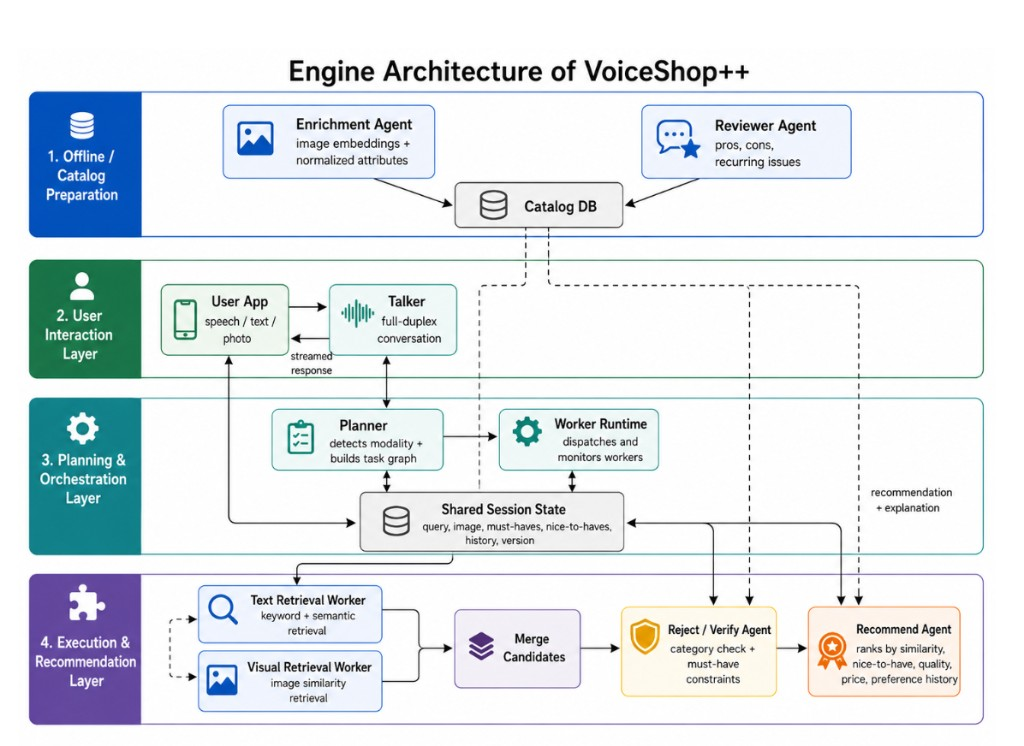
\includegraphics[width=\linewidth]{figures/engine_architecture.png}
  \caption{Engine architecture of VoiceShop++. Layer~1 (offline) writes reusable
  multimodal knowledge into the Catalog DB; Layer~2 handles full-duplex
  speech/text/photo interaction; Layer~3 plans and orchestrates the workers
  around a shared session state; Layer~4 executes retrieval, constraint
  verification and recommendation.}
  \label{fig:engine-arch}
\end{figure}

\begin{description}
  \item[Layer 1 --- Offline / Catalog Preparation.] Before any query is served,
  two offline agents enrich the catalog. The \emph{Enrichment Agent} converts
  each product image into a vector and a layer of normalised attributes, and the
  \emph{Reviewer Agent} distils raw customer reviews into structured pros, cons
  and recurring issues. Both persist their output into the Catalog DB so that the
  online path never pays their cost again.
  \item[Layer 2 --- User Interaction.] The user app accepts speech, text and
  photos; a full-duplex \emph{Talker} streams the conversation back to the user.
  \item[Layer 3 --- Planning \& Orchestration.] A \emph{Planner} detects the
  input modality and builds a task graph; a \emph{Worker Runtime} dispatches and
  monitors the workers. All agents communicate through a \emph{Shared Session
  State} that holds the query, image, must-haves, nice-to-haves, history and a
  version counter.
  \item[Layer 4 --- Execution \& Recommendation.] Text and Visual retrieval
  workers produce candidates that are merged, filtered by a \emph{Reject/Verify}
  agent (category and must-have constraints), and finally ordered by a
  \emph{Recommend} agent using similarity, nice-to-haves, quality, price and
  preference history.
\end{description}

The design is deliberately split into an \emph{offline} stage that materialises
expensive multimodal knowledge once, and an \emph{online} stage that is cheap,
LLM-light and robust. The remainder of this chapter presents the three technical
innovations that realise this design: (i)~offline multimodal catalog
preparation (Section~\ref{sec:innov-offline}); (ii)~text-plus-image retrieval in
a shared embedding space with modality-adaptive routing
(Section~\ref{sec:innov-retrieval}); and (iii)~a constraint-aware Reject/Verify
agent that decouples hard-constraint checking from soft-preference ranking
(Section~\ref{sec:innov-reject}).

\section{Innovation 1: Offline Multimodal Catalog Preparation}
\label{sec:innov-offline}

Raw e-commerce catalogs are sparse and single-modal: metadata is terse and
inconsistent, the product image is not searchable, and experiential knowledge is
buried in free-text reviews. The first innovation is to \emph{pre-compute}, once
and offline, a multimodal and constraint-checkable knowledge base attached to
each product. Two agents cooperate on this: the Enrichment Agent and the Reviewer
Agent, both writing into the Catalog DB.

\subsection{The Enrichment Agent}
\label{sec:enrichment}

Let the catalog be $\mathcal{C}=\{p_1,\dots,p_N\}$, where each product $p_i$ has
structured metadata and a remote image URL $u_i$. The Enrichment Agent
(\texttt{engine/enrichment.py}) materialises three artefacts per product.

\paragraph{(a) Image embedding in a shared space.}
We use a single multimodal embedding function
\begin{equation}
  \phi:\ \mathcal{X}_{\mathrm{img}}\cup\mathcal{X}_{\mathrm{txt}}\ \longrightarrow\ \mathbb{R}^{d},
  \label{eq:phi}
\end{equation}
provided by DashScope \texttt{multimodal-embedding-v1}, which maps \emph{both}
images and text into the \emph{same} $d$-dimensional space; this shared space is
what later makes cross-modal comparison meaningful. For product $p_i$ the agent
computes $\mathbf{v}_i=\phi(u_i)$ and stores it in the \texttt{image\_embedding}
column. Crucially, $u_i$ is sent to the service \emph{directly as a remote URL},
so the $\sim\!15\mathrm{k}$ catalog images are never downloaded to disk. Vectors
are serialised as Base64-encoded little-endian \texttt{float32} arrays, keeping
the catalog a single self-contained SQLite file.

\paragraph{(b) Source-aware attribute layering.}
Asking a vision--language model (VLM) to describe \emph{all} attributes is
unsafe, because a VLM hallucinates properties it cannot see (weight, battery,
price). We therefore introduce \textbf{source-aware attribute layering}: every
attribute is drawn only from the channel that can truthfully provide it
(Table~\ref{tab:layering}). The visual layer is extracted by Qwen-VL, prompted to
return \emph{only clearly visible} attributes and explicitly forbidden from
guessing physical or numeric properties; the physical layer is computed
deterministically from metadata (e.g.\ a \texttt{lightweight} flag from weight);
the textual layer summarises name and editorial fields. The three layers are
stored together as JSON in \texttt{visual\_attrs}.

\begin{table}[t]
  \centering
  \caption{Source-aware attribute layering. The visual model is never asked to
  guess physical or numeric properties, which curbs hallucination.}
  \label{tab:layering}
  \begin{tabular}{@{}lll@{}}
    \toprule
    \textbf{Layer} & \textbf{Source} & \textbf{Example attributes} \\
    \midrule
    Visual   & Qwen-VL on the image     & category, colours, style, shape, material look, pattern, keywords \\
    Physical & Structured metadata      & weight (+ \emph{lightweight} flag), battery, price, display \\
    Textual  & Name / summary / reasons & summary snippet, salient feature phrases \\
    \bottomrule
  \end{tabular}
\end{table}

\paragraph{(c) Enriched search text.}
From the layers the agent builds a single \texttt{enriched\_text} string $t_i$ by
concatenating the name, the searchable visual words (category, colours, style,
keywords, \dots), a few physical cues (``lightweight portable'', ``long
battery''), and the summary, after lower-cased de-duplication and truncation.
This string lets keyword search later match fine-grained attributes that never
appear in the terse product name (Section~\ref{sec:text}).

\paragraph{Robustness.}
Because enrichment depends on rate-limited third-party APIs, the agent fails
safely: (i)~embedding and VLM calls use bounded \emph{retry with exponential
back-off} to absorb transient $429$/network errors; (ii)~writes are
\emph{non-destructive} --- the vector is written only when a non-empty result is
returned, so a failed batch never wipes existing vectors, while the
metadata-derived attributes and enriched text are always written; and
(iii)~degradation is \emph{honest} --- on the online path a failed embedding
leaves the field empty (and hence visible) rather than substituting a fake
vector. Algorithm~\ref{alg:enrich} summarises the procedure; a guard
\textproc{HasEnrichment} reports whether any vector exists, which the online
layer uses to decide whether visual retrieval is available.

\begin{algorithm}[t]
\caption{Offline catalog enrichment (per product)}
\label{alg:enrich}
\begin{algorithmic}[1]
\Require product $p_i$ with image URL $u_i$ and metadata $m_i$
\State $\mathbf{v}_i \gets \phi(u_i)$ \Comment{embed remote URL; $\varnothing$ on failure}
\State $a^{\mathrm{vis}} \gets \textproc{QwenVL}(u_i)$ \Comment{visible attributes only}
\State $a^{\mathrm{phy}} \gets \textproc{PhysicalFromMeta}(m_i)$;\quad
       $a^{\mathrm{txt}} \gets \textproc{TextualFromMeta}(m_i)$
\State $t_i \gets \textproc{BuildEnrichedText}(m_i, a^{\mathrm{vis}}, a^{\mathrm{phy}})$
\If{$\mathbf{v}_i \neq \varnothing$}
  \State write \texttt{image\_embedding}, \texttt{visual\_attrs}, \texttt{enriched\_text}
\Else
  \State write \texttt{visual\_attrs}, \texttt{enriched\_text} \Comment{preserve old vector}
\EndIf
\end{algorithmic}
\end{algorithm}

\subsection{The Reviewer Agent}
\label{sec:reviewer}

Many experiential requirements --- ``the fan is quiet'', ``breathable in
summer'', ``runs true to size'' --- appear \emph{only} in customer reviews. The
Reviewer Agent (\texttt{engine/reviewer.py}) turns raw reviews into structured,
verifiable knowledge. In our design reviews serve \emph{verification and
explanation}, not recall; retrieval is left to the text and image channels, so
the agent produces aspect-level attributes but \emph{no} review embedding.

\paragraph{Aggregation with quality weighting.}
Reviews are read from the Amazon Reviews 2023 dumps~\cite{hou2024bridging} and grouped by
\texttt{parent\_asin}, the catalog primary key. For product $p_i$ with review set
$R_i$, each review $r$ receives a quality score
\begin{equation}
  q(r)=\alpha\,\ind[\text{verified}]
       +\beta\,\mathrm{helpful\_votes}(r)
       +\gamma\,\ind[\text{non-empty text}],
  \label{eq:quality}
\end{equation}
and the top reviews (up to a per-product cap) are concatenated, highest quality
first, so the language model reasons over trustworthy, information-dense text.

\paragraph{Aspect-based extraction.}
From the aggregate text an LLM (Qwen, constrained to JSON) extracts
\begin{equation}
  \mathrm{aspects}(p_i)=\{\textsf{pros},\ \textsf{cons},\ \textsf{issues},\
  \textsf{aspects},\ \textsf{summary},\ \textsf{keywords}\},
  \label{eq:aspects}
\end{equation}
where \textsf{aspects} maps named facets (comfort, battery, sizing, \dots) to a
sentiment and \textsf{keywords} collects the adjectives buyers repeatedly use.
When no LLM is available, a deterministic word-frequency and adjective heuristic
still guarantees non-empty keywords, so the pipeline never blocks. The result is
stored as JSON in \texttt{review\_aspects} with \texttt{review\_count\_used};
writes are non-destructive. This knowledge is consumed online by the
Reject/Verify agent of Section~\ref{sec:innov-reject}, where review keywords and
pros let a soft requirement that lives only in reviews still be matched against a
candidate.

\section{Innovation 2: Text-plus-Image Retrieval}
\label{sec:innov-retrieval}

The second innovation is a retrieval stage that draws on \emph{both} the enriched
text and the image vectors of Section~\ref{sec:innov-offline}, and that is
composed adaptively according to what the user actually provided. Two workers ---
Text Retrieval and Visual Retrieval --- run in parallel and their outputs are
fused.

\subsection{Text retrieval}
\label{sec:text}

The user request is first turned into a preference profile by an upstream
analysis LLM, whose English \emph{search keywords} $K_q$ are the primary query
signal (so a Chinese or spoken request can still search the English catalog). The
Text Retrieval worker (\texttt{engine/worker/search\_worker.py} with the catalog
\texttt{search} function) forms a query string from $K_q$, applies a budget-based
price ceiling and a platform post-filter, and tokenises the query into a content
token set $Q$ (length $\geq 3$, stop-words removed, de-duplicated, capped). A
product is recalled if any token matches its name \emph{or}, when enrichment is
available, its enriched text:
\begin{equation}
  \mathrm{recall}(p_i)=\bigvee_{k\in Q}
  \big(k \sqsubseteq \mathrm{name}(p_i)\ \lor\ k \sqsubseteq t_i\big),
  \label{eq:text-recall}
\end{equation}
where $\sqsubseteq$ denotes substring (\texttt{LIKE}) containment. Matching
against $t_i$ is the payoff of the enrichment layer: fine-grained visual and
experiential terms become searchable even though they are absent from the product
name. Candidates are then ranked by a name-relevance score
\begin{equation}
  \mathrm{rel}(p_i)=\sum_{k\in Q}\ind\!\left[k\sqsubseteq\mathrm{name}(p_i)\right],
  \label{eq:rel}
\end{equation}
with ties broken by popularity, rating or price. Anchoring the relevance term to
the name while letting recall fire on the broader enriched text keeps precision
tied to the most reliable field while enrichment only \emph{expands} coverage.
Category is intentionally \emph{not} a hard filter here: recall stays high and
category precision is delegated to the Reject/Verify agent
(Section~\ref{sec:innov-reject}).

\subsection{Visual retrieval}
\label{sec:photo}

The Visual Retrieval worker (\texttt{visual\_recall} in
\texttt{engine/enrichment.py}) retrieves products whose image is visually similar
to a user photo. On first use it loads all stored vectors into an in-memory
\texttt{VisualIndex} (ids, vectors $\{\mathbf{v}_i\}$, and categories parsed from
the visual layer); the index is cached across requests and invalidated on
re-enrichment. Given a user photo $I_q$, every product is scored by cosine
similarity in the shared space,
\begin{equation}
  s^{\mathrm{vis}}_i=\cos\!\big(\phi(I_q),\,\mathbf{v}_i\big),
  \qquad
  \cos(\mathbf{a},\mathbf{b})=\frac{\mathbf{a}^{\top}\mathbf{b}}{\lVert\mathbf{a}\rVert\,\lVert\mathbf{b}\rVert},
  \label{eq:svis}
\end{equation}
computed in pure Python (no numerical dependency); a zero or dimension-mismatched
operand yields $0$, so malformed vectors never raise errors. When a target
category $c$ is known --- for example inferred by the VLM from the photo in the
image-only modality --- a \emph{category guardrail} restricts scoring to
compatible products, preventing visually-similar but categorically-wrong matches:
\begin{equation}
  \mathrm{VisualRecall}(I_q)=\operatorname*{top\text{-}K}_{\,i\,:\,\mathrm{cat}_i\sim c}\ s^{\mathrm{vis}}_i .
  \label{eq:vrecall}
\end{equation}
Each returned product is annotated with its \texttt{\_visual\_score}
(Algorithm~\ref{alg:vrecall}).

\begin{algorithm}[t]
\caption{Online visual recall}
\label{alg:vrecall}
\begin{algorithmic}[1]
\Require user photo $I_q$, optional category $c$, index $\{(\text{id}_i,\mathbf{v}_i,\mathrm{cat}_i)\}$
\If{index is empty} \Return $\varnothing$ \EndIf
\State $\mathbf{q}\gets\phi(I_q)$
\State $S \gets \{(\text{id}_i,\ \cos(\mathbf{q},\mathbf{v}_i)) : c\text{ unset}\ \lor\ \mathrm{cat}_i\sim c\}$
\State sort $S$ descending by score;\ \Return top-$K$, attaching \texttt{\_visual\_score}
\end{algorithmic}
\end{algorithm}

\subsection{Fusion and modality-adaptive routing}
\label{sec:fusion}

The Recall agent (\texttt{engine/worker/recall\_worker.py}) merges the two
channels by an order-preserving union that keeps the first occurrence of each
product id (keyword hits first, visual hits supplementing). It then attaches a
visual score to \emph{every} surviving candidate --- including those recalled
only by text --- so that a downstream ranker sees a uniform $s^{\mathrm{vis}}$
signal regardless of the channel of origin, enabling fair multimodal fusion.

Which channels run is decided per request by a modality router that classifies
the input as text-only ($T$), text-plus-image ($T{+}I$), or image-only ($I$):
$T$ runs text retrieval only; $T{+}I$ runs both channels and merges; $I$ first
infers a category from the photo and then runs category-guarded visual
retrieval. Every channel is independently switchable through an experiment
configuration, so the contribution of enrichment and of visual recall can be
measured by ablation. Visual retrieval is strictly additive: it activates only
when a query image is present \emph{and} the catalog contains vectors, and
otherwise the pipeline proceeds on text alone.

\section{Innovation 3: The Reject/Verify Agent}
\label{sec:innov-reject}

Recall is tuned for coverage, not precision, so the merged candidate set contains
items that are visually or lexically similar yet violate a hard requirement
(wrong category, over budget, missing a must-have feature). The third innovation
inserts an independent \emph{Reject/Verify} agent (\texttt{engine/verifier.py})
between recall and ranking, which \textbf{decouples hard-constraint checking from
soft-preference ranking}: the verifier only decides \emph{keep} or \emph{reject},
while the ordering of survivors is left entirely to the Recommend agent. This
separation of concerns keeps each stage simple and independently ablatable.

\paragraph{Two-tier decision.}
The agent applies a cheap, reliable \emph{rule pre-filter} to every candidate
using only trustworthy structured fields --- rejecting items that are clearly
over budget (with a rough currency conversion) or on the wrong platform. The
survivors are then checked for the two core hard constraints: (i)~\emph{category
consistency} with the user's desired category and (ii)~\emph{satisfaction of all
must-haves}. This check can run as a rule-based matcher or, by default, as an
LLM-as-Judge.

\paragraph{Constraint-aware evidence.}
For the rule matcher, each candidate is flattened into a textual ``haystack''
that deliberately aggregates evidence from \emph{all} offline layers: the name
and summary, the \texttt{enriched\_text} and \texttt{visual\_attrs} from the
Enrichment Agent, and the keywords, pros and summary from the Reviewer Agent's
\texttt{review\_aspects}. A category or must-have token is deemed satisfied when
it matches this haystack, so an experiential must-have that exists only in
reviews (``quiet'', ``breathable'') can still be verified --- directly
connecting Innovation~1 to constraint checking.

\paragraph{LLM-as-Judge.}
In the default mode, up to a bounded number of candidates are sent in a single
batched call to a judge LLM that returns, per candidate, a
\texttt{category\_match}, a \texttt{must\_haves\_met} verdict and a keep/reject
decision with a short reason; candidates beyond the budget, or all candidates
when the LLM is unavailable, fall back to the rule matcher. Batching bounds the
online LLM cost, and the graceful fallback guarantees the gate always produces a
decision.

\paragraph{Unknown-tolerance.}
A distinctive design choice is \emph{unknown-tolerance}: when an attribute cannot
be determined from the available information, the default policy treats it as
``not violated'' and keeps the candidate, rather than rejecting on missing
evidence. This avoids the failure mode where an over-strict gate empties the
result set. The behaviour is configurable through an ablation switch with four
settings --- \texttt{off} (no verification), \texttt{rule} (rules only),
\texttt{llm\_strict} (LLM judge, reject on unknown), and \texttt{llm} (LLM judge
with unknown-tolerance, the default) --- so the precision/recall trade-off of the
gate can be studied directly. The agent returns both the kept set and the
rejected items with reasons, the latter feeding the user-facing explanation
(``recommendation + explanation'' in Figure~\ref{fig:engine-arch}).

\section{Summary}
\label{sec:engine-summary}

The three innovations compose into a coherent engine: Innovation~1 turns a
sparse, image-only catalog into a multimodal, constraint-checkable knowledge base
offline; Innovation~2 serves it through text and image retrieval in a shared
embedding space, composed adaptively to the input modality; and Innovation~3
guarantees that only candidates satisfying the user's hard constraints reach the
ranker, while reusing all offline knowledge as verification evidence.
Table~\ref{tab:agent-summary} summarises the agents involved. Throughout, a
consistent set of principles --- a shared embedding space, source-aware attribute
layering, non-destructive materialisation, and honest graceful degradation ---
keeps the system correct and robust under unreliable external services.

\begin{table}[t]
  \centering
  \caption{The catalog and retrieval agents at a glance.}
  \label{tab:agent-summary}
  \begin{tabular}{@{}llll@{}}
    \toprule
    \textbf{Agent} & \textbf{Innovation / Stage} & \textbf{Reads} & \textbf{Writes / Returns} \\
    \midrule
    Enrichment      & 1 (offline) & image URL, metadata               & \texttt{image\_embedding}, \texttt{visual\_attrs}, \texttt{enriched\_text} \\
    Reviewer        & 1 (offline) & Amazon reviews                    & \texttt{review\_aspects}, \texttt{review\_count\_used} \\
    Text Retrieval  & 2 (online)  & keywords, \texttt{enriched\_text} & ranked candidates (name relevance) \\
    Visual Retrieval& 2 (online)  & query photo, \texttt{image\_embedding} & ranked candidates ($\texttt{\_visual\_score}$) \\
    Reject/Verify   & 3 (online)  & candidates + all offline layers   & kept set, rejected + reasons \\
    \bottomrule
  \end{tabular}
\end{table}
